\subsection{a}
Given that we want 20 steps of size 0.1, we center the polynomial around $20 \cdot 0.1 = 2$.
We also calculate the integral of the expression, as seen in the matlab code.
\lstinputlisting[caption={Topic 8. Question a}]{"./files/topic8/a.m"}

\texttt{p(end)} evaluates to 0.0364

\pagebreak
\subsection{b}

\lstinputlisting[caption={Topic 8. Question b}]{"./files/topic8/b.m"}

\texttt{yb(end)} evaluates to 0.0107

\subsection{c}

By inspection we find that $y(t) = -\frac{1}{4} \cos\left(4t\right)$, and therefore $y(2) = 0.0364$.
As expected, the taylor polynomial gave us a similar answer; however if we look at Figure \ref{fig:taylor}, a period cannot be deduced.
On the other hand, Euler's method, Figure \ref{fig:euler}, gives us an inaccurate value (0.0107), but a very good shape for the graph -- from which we can estimate the period to be 1.5.
From the equation we know the period to be $\frac{2\pi}{4} \approx 1.57$.
\begin{figure}[h]
    \centering
    \begin{minipage}{0.45\textwidth}
        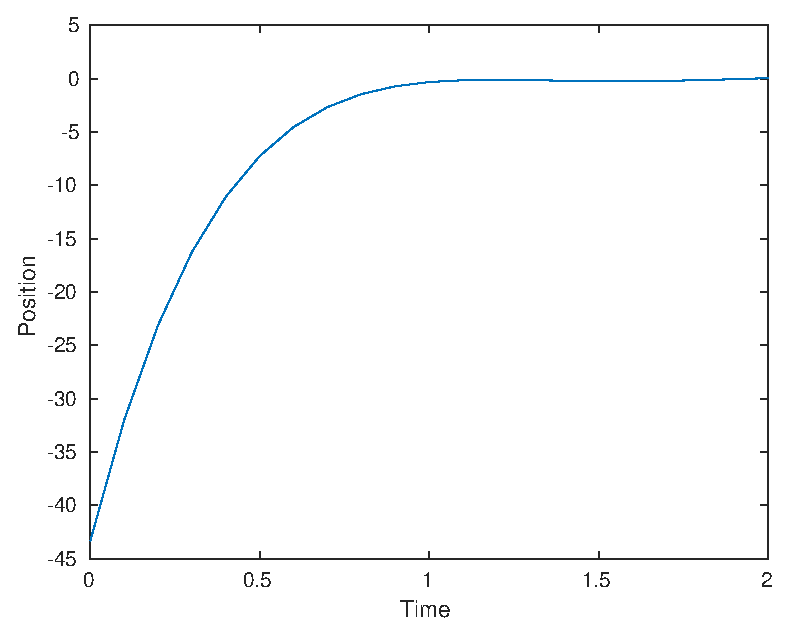
\includegraphics[scale=0.55, center]{./eps/topic8_a.eps}
        \caption{Taylor polynomial centered around 2.}
        \label{fig:taylor}
    \end{minipage}
    \begin{minipage}{0.45\textwidth}
        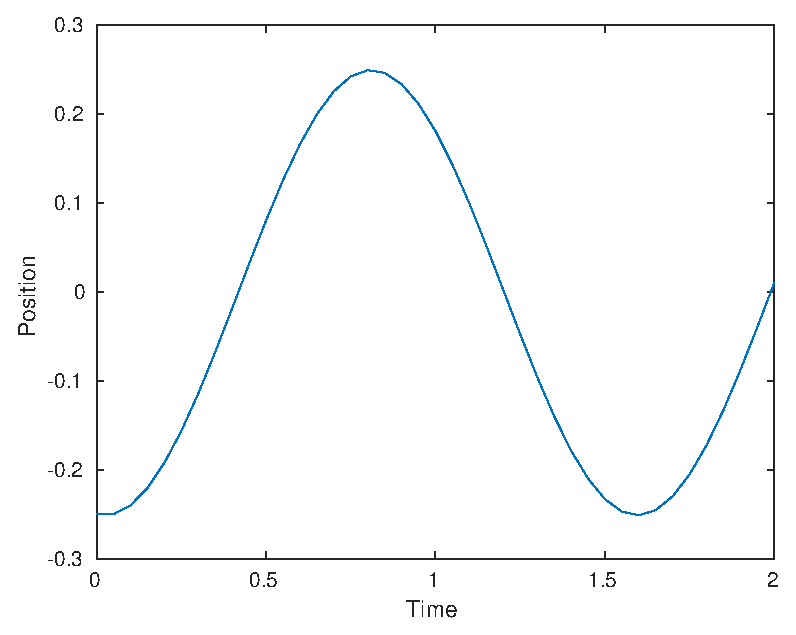
\includegraphics[scale=0.55, center]{./eps/topic8_b.eps}
        \caption{Euler method.}
        \label{fig:euler}
    \end{minipage}
    \label{}
\end{figure}

By increasing the order of the Taylor polynomial, we are able to reduce this difference significantly.
Below is the same expression with order 100, which can be seen to have a similar shape to Euler's method and more appropriate values.
\begin{figure}[h]
    \centering
    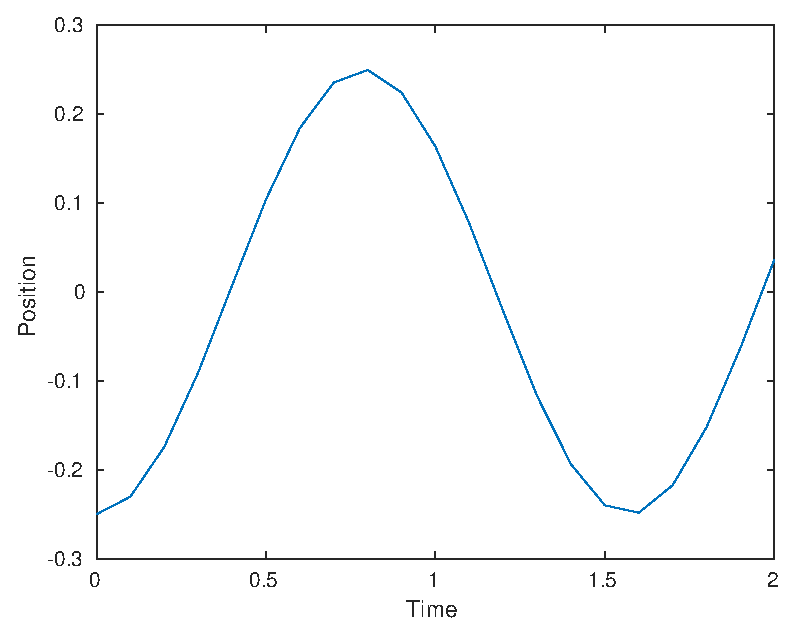
\includegraphics[scale=0.65, center]{eps/topic8_c.eps}
    \caption{Taylor polynomial with high order.}
    \label{fig:taylorOrder100}
\end{figure}
\lstinputlisting[caption={Taylor polynomial of order 100}]{"./files/topic8/c.m"}